
% Also note that the "draftcls" or "draftclsnofoot", not "draft", option
% should be used if it is desired that the figures are to be displayed in
% draft mode.
%
%\documentclass[12pt, draftclsnofoot, onecolumn]{IEEEtran}
\documentclass[conference, twocolumn]{IEEEtran}

%\usepackage[latin1]{inputenc} % Latin1
\usepackage[utf8]{inputenc} 	% UTF-8

%\usepackage{amsmath,amsthm}
\usepackage{amssymb}
%\usepackage{amsfonts}
\usepackage{bbm} % For indicator function
%\usepackage{breeq}
\usepackage{graphicx}
\usepackage{color,psfrag}


% Dashed arrow and control the size of the braces due to underbrace
\usepackage{MnSymbol}
%\graphicspath{{./figures/}}

%Strike out the sentence
\usepackage[normalem]{ulem}

% Draw something blocks or ovelap
\usepackage{tikz}
\usepackage{siunitx}
\usepackage{cite} % Combining multiple citations

\usepackage{longtable}

\usepackage{xcolor}
\newcommand{\tc}[1]{#1}
%\newcommand{\tc}[1]{\textcolor[rgb]{0.0,0.0,1.0}{#1}}
% Flush all figures and tables at the end of the document
%\usepackage[nolists, nomarkers]{endfloat}

%% Placing the footnote in figure caption
%\usepackage{ftnxtra}
%\usepackage{fnpos} % \makeFNbelow by default



\newcommand{\e}[2]{{\mathbb E}_{#1}\left[ #2 \right]}
\newcommand{\s}[2]{{\frac{1}{{#1}}\sum_n^{#1}} {#2}}
\newcommand{\q}[3]{{\mathcal Q}_{#1}\left( #2 \right)}
\newcommand{\p}{\mathbb P}
\newcommand{\sub}[1]{_{\text{#1}}}
\newcommand{\pd}{\text{P}\sub{d}}
\newcommand{\op}{\text{P}\sub{out}}
\newcommand{\opc}{\rho\sub{out}}
\newcommand{\pc}{P\sub{Tx,ST,full}}
\newcommand{\pdd}{\bar{\text{P}}\sub{d}}
\newcommand{\preg}{P\sub{Tx,ST,cont}}
\newcommand{\xreg}{x\sub{ST,cont}}
\newcommand{\prcvd}{P\sub{Rx,ST}}
\newcommand{\prcvdsr}{P\sub{Rx,SR}}
\newcommand{\eprcvd}{\hat{P}\sub{Rx,ST}}
\newcommand{\eprcvdsr}{\hat{P}\sub{Rx,SR}}
\newcommand{\yrcvd}{y\sub{ST}}
\newcommand{\ptran}{P\sub{Tx,PR}}
\newcommand{\ptranpt}{P\sub{Tx,PT}}
\newcommand{\xtran}{x\sub{PR}}
\newcommand{\xtranpt}{x\sub{PT}}
\newcommand{\pp}{P\sub{Rx,PR}}
\newcommand{\yp}{y\sub{PR}}
\newcommand{\ys}{y\sub{SR}}
\newcommand{\nap}{w\sub{PR}}
\newcommand{\nas}{w\sub{ST}}
\newcommand{\nasr}{w\sub{SR}}
\newcommand{\ite}{\theta\sub{I}}
\newcommand{\rs}{R\sub{s}}
\newcommand{\trs}{R\sub{s}}
\newcommand{\ers}{\e{}{\rs}}
%\newcommand{\gp}{g\sub{p}}
\newcommand{\gpo}{h\sub{PR,ST}}
\newcommand{\gpt}{h\sub{PT,SR}}
\newcommand{\egpo}{\hat{h}\sub{PR,ST}}
\newcommand{\egpt}{\hat{h}\sub{PT,SR}}
\newcommand{\epgpo}{|\hat{h}\sub{PR,ST}|^2}
\newcommand{\epgpt}{|\hat{h}\sub{PR,SR}|^2}
\newcommand{\epgs}{|\hat{h}\sub{ST,SR}|^2}
\newcommand{\gs}{h\sub{ST,SR}}
\newcommand{\pgpo}{|h\sub{PR,ST}|^2}
\newcommand{\pgpt}{|h\sub{PT,SR}|^2}
\newcommand{\egs}{\hat{h}\sub{s}}
\newcommand{\pgs}{|h\sub{ST,SR}|^2}
\newcommand{\bpgpo}{|\bar{h}\sub{PR,ST}|^2}
\newcommand{\bpgpt}{|\bar{h}\sub{PT,SR}|^2}
\newcommand{\bpgs}{|\bar{h}\sub{ST,SR}|^2}
%\newcommand{\ap}{\alpha\sub{p}}
%\newcommand{\apt}{\alpha\sub{p}}
\newcommand{\npp}{\sigma^2\sub{p}}
\newcommand{\nps}{\sigma^2}
\newcommand{\npu}{\Delta\sigma^2}
\newcommand{\fsam}{f\sub{s}}
\newcommand{\ttau}{\tilde{\tau}}
\newcommand{\ca}{\text{C}\sub{s}}
\newcommand{\eca}{\hat{\text{{C}}}\sub{s}}
\newcommand{\mpo}{m\sub{PR,ST}}
\newcommand{\mpt}{m\sub{PT,SR}}
\newcommand{\ms}{m\sub{ST,SR}}

% distribution functions
\newcommand{\fpreg}{F_{\preg}}
\newcommand{\fprcvd}{F_{\eprcvd}}
\newcommand{\fpgpo}{F_{\pgpo}}
\newcommand{\fpgpt}{F_{\pgpt}}
\newcommand{\fpgs}{F_{\pgs}}
\newcommand{\fprcvdsr}{F_{\eprcvdsr}}
\newcommand{\fpp}{F_{\pp}}
\newcommand{\frs}{F_{\rs}}
\newcommand{\fgs}{F_{\epgs}}
\newcommand{\fgp}{F_{\epgpo}}
\newcommand{\fc}{F_{\eca}}

% density functions
\newcommand{\dprcvd}{f_{\prcvd}}
\newcommand{\dK}{f_{\gpo \prcvd}}
\newcommand{\dpp}{f_{\pp}}
\newcommand{\dpreg}{f_{\preg}}
\newcommand{\drs}{f_{\rs}}
\newcommand{\dgp}{f_{\epgpo}}
\newcommand{\dgs}{f_{\epgs}}
\newcommand{\dc}{f_{\eca}}

\newcommand{\lpo}{\lambda\sub{p,1}}
\newcommand{\lpt}{\lambda\sub{p,2}}
\newcommand{\ls}{\lambda\sub{s}}
\newcommand{\Ks}{\tau\sub{p}{\fsam}}

\newcommand{\apo}{a\sub{p,1}}
\newcommand{\bpo}{b\sub{p,1}}
\newcommand{\apt}{a\sub{p,2}}
\newcommand{\bpt}{b\sub{p,2}}
\newcommand{\as}{a\sub{s}}
\newcommand{\bs}{b\sub{s}}
\newcommand{\tp}{\frac{\tau\sub{p}}{2}}

\newcommand{\imp}{\uline}
\newcommand{\ur}{\uuline}
\newcommand{\ns}{\uwave} 
\newcommand{\ws}{\sout}
\newcommand{\fl}{\dashuline}
\newcommand{\un}{\dotuline}
\DeclareMathOperator*{\Pro}{Pr}
\DeclareMathOperator*{\maxi}{max}
\DeclareMathOperator*{\expec}{\mathbb{E}}
\DeclareMathOperator*{\gthan}{\ge}
\DeclareMathOperator*{\eqto}{=}
\DeclareMathOperator*{\cosi}{ci}
\DeclareMathOperator*{\sini}{si}
\DeclareMathOperator*{\iGamma}{\text{inv}-\Gamma}
\DeclareMathOperator*{\ncchi2}{{\mathcal{X}\sp{\prime}}^2}
\DeclareMathOperator*{\invncchi2}{\text{}\mathcal{X'}^2}


\newtheorem{theorem}{\tc{Problem}}
\newtheorem{case}{Case}
\newtheorem{constraint}{Constrai3}
\newtheorem{lemma}{Lemma}
\newtheorem{prop}{Proposition}
\newtheorem{remark}{Remark}
\newtheorem{coro}{Corollary}
\newtheorem{defi}{Definition}
\newtheorem{approxi}{Approximation}
%\DeclareGraphicsExtensions{.pdf}

% correct bad hyphenation here
%\hyphenation{net-works hop-set}
\makeatletter
\if@twocolumn
	\newcommand{\figscale}{0.92 \columnwidth}
	\newcommand{\figscalet}{\columnwidth}
	\newcommand{\figscalett}{\columnwidth}
\else
	\newcommand{\figscale}{0.44 \columnwidth}
	\newcommand{\figscalet}{0.46 \columnwidth}
	\newcommand{\figscalett}{0.68 \columnwidth}
\fi
\makeatother


\makeatletter
\if@twocolumn
	\newcommand{\figmara}{0mm}
	\newcommand{\figmarb}{-2mm}
	\newcommand{\figmarc}{0mm}
	\newcommand{\figmard}{0mm} % margin between figure and caption matlab and single 
	\newcommand{\subfigmar}{4mm}
	\newcommand{\tablespacing}{1.4}
	\newcommand{\tmara}{-0.0cm}
	\newcommand{\tmarb}{-0.0cm}
	\newcommand{\absmara}{-0.0cm}
	\newcommand{\absmarb}{-0.0cm}
	\newcommand{\keymara}{-0.0cm}
	\newcommand{\keymarb}{-0.0cm}
\else
	\newcommand{\figmara}{-4mm}
	\newcommand{\figmarb}{-10mm}
	\newcommand{\figmarc}{-5mm} % margin between figure and caption gimp figures
	\newcommand{\figmard}{-3mm} % margin between figure and caption matlab and single 
	\newcommand{\subfigmar}{2mm}
	\newcommand{\tablespacing}{0.85}
	\newcommand{\tmara}{-0.6cm}
	\newcommand{\tmarb}{-0.4cm}
	\newcommand{\absmara}{-2.0cm}
	\newcommand{\absmarb}{-0.2cm}
	\newcommand{\keymara}{-0.3cm}
	\newcommand{\keymarb}{-0.3cm}
\fi
\makeatother


% Subfigures
\ifCLASSOPTIONcompsoc
\usepackage[caption=false,font=normalsize,labelfont=sf,textfont=sf]{subfig}
\else
\usepackage[caption=false,font=footnotesize]{subfig}
\fi

% Metadata
%\usepackage[final=true]{hyperref}
%\hypersetup{
%	pdfauthor = {Ankit Kaushik et al.},
%	pdftitle = {CrownCom 2015},
%	pdfsubject = {CrownCom 2015},
%	pdfcreator = {PDFLaTeX with hyperref package},
%	pdfproducer = {PDFLaTeX}
%	hidelinks = {true}
%}


% Used to break the theorems, proof between the columns
%\allowdisplaybreaks

%used to equalize the last pages
%\usepackage{flushend}

\begin{document}
%
\title{Performance Analysis of Interweave Cognitive Radio Systems with Imperfect Channel Knowledge over Nakagami Fading Channels}
\author{\IEEEauthorblockN{Ankit Kaushik\IEEEauthorrefmark{1}, Shree Krishna Sharma\IEEEauthorrefmark{2}, Symeon Chatzinotas\IEEEauthorrefmark{2},  Bj\"orn Ottersten\IEEEauthorrefmark{2}, Friedrich Jondral\IEEEauthorrefmark{1}}
\IEEEauthorblockA{\IEEEauthorrefmark{1}Communications Engineering Lab, Karlsruhe Institute of Technology (KIT), Germany}
\{ankit.kaushik, friedrich.jondral\}@kit.edu
\IEEEauthorblockA{\IEEEauthorrefmark{2}SnT - securityandtrust.lu, University of Luxembourg, Luxembourg}
\{shree.sharma, symeon.chatzinotas, bjorn.ottersten\}@uni.lu
\thanks{This work was partially supported by the National Research Fund, Luxembourg under the CORE projects ``SeMIGod'' and ``SATSENT''.}
}

% make the title area
\maketitle
\thispagestyle{empty}
\pagestyle{empty}


\vspace{-1.7cm}

Over the last decade, wireless communication is witnessing a tremendous growth in the data traffic due to ever-increasing number of connected devices. According to the recent surveys on mobile traffic by prominent market leaders (Cisco \cite{CISCO14} and Ericsson\cite{Eric15}), the existing mobile traffic is expected to increase $11$-fold  by 2021. Certainly, in future, the state-of-the-art standards (fourth-Generation (4G) -- LTE, WiMAX) are incapable of sustaining the substantial amount of data traffic, originating from these devices. It is being visualized that a major portion of this requirement can be satisfied through an additional spectrum. Due to exclusive usage, the spectrum below $\SI{6}{GHz}$ is not able to meet this demand of additional spectrum, leading to its scarcity. To this end, Cognitive Radio (CR), along with millimeter-wave technology \cite{Rapp13} and visible-light communication \cite{Wu14}, is envisaged as an alternative source of spectrum. The latter techniques are limited to a point-to-point communication, by which mobility is compromised. In contrast, a CR system aims at an efficient utilization of the spectrum below $\SI{6}{GHz}$ -- suitable for mobile communications -- by enabling a secondary access to the licensed spectrum while ensuring a sufficient protection to the licensed users (also referred as a primary system).

Despite the fact that an extensive amount of literature -- including \cite{Liang08, Kang209, Kang09} -- has been dedicated to the field of CR, its performance analysis has been dealt inadequately from a deployment perspective. Therefore, making it difficult to understand the extent of vulnerability caused to the primary system. In this context, it is essential to establish a deployment-centric viewpoint for analyzing the performance of a CR system. Following this viewpoint, it has been identified that the involved channels' knowledge at the secondary transmitter is pivotal for the realization of cognitive techniques. However, the aspect of channel knowledge in context to CR systems, particularly its impact on the performance, has not been clearly understood. With the purpose of curtailing this gap, the research carried out at Communications Engineering Lab (CEL), Karlsruhe Institute of Technology (KIT) proposes a successful integration of this knowledge -- by carrying out channel estimation -- in reference to different CR systems, namely interweave, underlay and hybrid systems. More specifically, our work outlines the following aspects corresponding to the aforementioned CR systems, employing different cognitive techniques such as spectrum sensing, power control and their combination.

\subsection*{Analytical Framework}
First, an analytical framework is established to characterize the effects such as time allocation and variation, arising due to the incorporation of imperfect channel knowledge, that are detrimental to the performance of the CR systems \cite{Kaushik16_TWC, Kaushik16_TCCN}. 

In order to satisfy the low complexity and the versatility towards unknown primary user signal requirements, which are necessary for the deployment of the CR systems, a received power-based channel estimation is included in the proposed framework. In this regard, an effort has been made to facilitate a direct incorporation of the estimated parameter (received power) to the performance characterization of the CR systems.
%In order to facilitate hardware deployment of a CR system, received power-based estimation, a novel channel estimation technique is employed for the channels existing between the primary and the secondary systems, thus fulfilling low-complexity and versatility requirements.

Besides, a stochastic approach is followed for characterizing the variations in the system. In particular, these variations cause uncertainty in the interference power received at the primary system, which may completely disrupt the operation of the CR systems. In order to maintain this uncertainty below a desired level, new interference constraints are proposed. %Moreover, the theoretical expressions, derived for the performance evaluation, are verified by means of simulations.


%specially for the channels between the primary and secondary systems. 
%In this context, the proposed framework captures the performance degradation, due to time allocated for performing channel estimation and the imperfect knowledge, the performance with the baseline models, constituting perfect channel knowledge. 

\captionsetup[subfigure]{position=top}
\begin{figure}[!ht]
\centering
\subfloat[]{
%% Add psfrag entries
\input{figures/fig_opt_thr_vs_est_time_sen_time_oc_AWGN.tex}
\centering
\begin{tikzpicture}[scale=1]
\node[anchor=south west,inner sep=0] (image) at (0,0)
{
\includegraphics[width= \figscale]{figures/fig_opt_thr_vs_est_time_sen_time_oc_AWGN}
};
\begin{scope}[x={(image.south east)},y={(image.north west)}]
%\draw[black,->] (0.6,0.44) node[above=0.0,  font=\scriptsize] {$\mpd \in \{0.05,0.10,0.15\}$} -- (0.56,0.33);
\draw[black,->] (0.353,0.83) -- (0.353,0.699);
\node[draw=none, font=\scriptsize] at (0.353, 0.86) {$\rs(\ttest, \ttsen)$};

%\draw[help lines,xstep=.1,ystep=.1] (0,0) grid (1,1);
%\foreach \x in {0,1,...,9} { \node [anchor=north] at (\x/10,0) {0.\x}; }
%\foreach \y in {0,1,...,9} { \node [anchor=east] at (0,\y/10) {0.\y}; }
\end{scope}
\end{tikzpicture}
\label{fig_IS:PT}
}
\vspace{4mm}
\hfil
\subfloat[]{
% This file is generated by the MATLAB m-file laprint.m. It can be included
% into LaTeX documents using the packages graphicx, color and psfrag.
% It is accompanied by a postscript file. A sample LaTeX file is:
%    \documentclass{article}\usepackage{graphicx,color,psfrag}
%    \begin{document}% This file is generated by the MATLAB m-file laprint.m. It can be included
% into LaTeX documents using the packages graphicx, color and psfrag.
% It is accompanied by a postscript file. A sample LaTeX file is:
%    \documentclass{article}\usepackage{graphicx,color,psfrag}
%    \begin{document}\input{fig_thr_est_time_tradeoff_AWGN}\end{document}
% See http://www.mathworks.de/matlabcentral/fileexchange/loadFile.do?objectId=4638
% for recent versions of laprint.m.
%
% created by:           LaPrint version 3.16 (13.9.2004)
% created on:           05-Feb-2015 04:59:16
% eps bounding box:     14 cm x 10.5 cm
% comment:              
%
%\begin{psfrags}%
%\psfragscanon%
%
% text strings:
\psfrag{s08}[b][b]{\fontsize{9}{13.5}\fontseries{m}\mathversion{normal}\fontshape{n}\selectfont \color[rgb]{0,0,1}\setlength{\tabcolsep}{0pt}\begin{tabular}{c}$\ers$ = [bits/sec/Hz]\end{tabular}}%
\psfrag{s09}[t][t]{\fontsize{9}{13.5}\fontseries{m}\mathversion{normal}\fontshape{n}\selectfont \color[rgb]{0,0,0}\setlength{\tabcolsep}{0pt}\begin{tabular}{c}$\tau$ = [ms]\end{tabular}}%
\psfrag{s13}[][]{\fontsize{10}{15}\fontseries{m}\mathversion{normal}\fontshape{n}\selectfont \color[rgb]{0,0,0}\setlength{\tabcolsep}{0pt}\begin{tabular}{c} \end{tabular}}%
\psfrag{s14}[][]{\fontsize{10}{15}\fontseries{m}\mathversion{normal}\fontshape{n}\selectfont \color[rgb]{0,0,0}\setlength{\tabcolsep}{0pt}\begin{tabular}{c} \end{tabular}}%
\psfrag{s16}[t][t]{\fontsize{9}{13.5}\fontseries{m}\mathversion{normal}\fontshape{n}\selectfont \color[rgb]{0,0.5,0}\setlength{\tabcolsep}{0pt}\begin{tabular}{c}$\pc$\end{tabular}}%
\psfrag{s17}[t][t]{\fontsize{9}{13.5}\fontseries{m}\mathversion{normal}\fontshape{n}\selectfont \color[rgb]{0,0,0}\setlength{\tabcolsep}{0pt}\begin{tabular}{c}$\tau$ = [ms]\end{tabular}}%
\psfrag{s18}[l][l]{\fontsize{9}{13.5}\fontseries{m}\mathversion{normal}\fontshape{n}\selectfont \color[rgb]{0,0,0}sim}%
\psfrag{s19}[l][l]{\fontsize{9}{13.5}\fontseries{m}\mathversion{normal}\fontshape{n}\selectfont \color[rgb]{0,0,0}(6)}%
\psfrag{s20}[l][l]{\fontsize{9}{13.5}\fontseries{m}\mathversion{normal}\fontshape{n}\selectfont \color[rgb]{0,0,0}$\pc$, $\npu$ = 0 dB}%
\psfrag{s21}[l][l]{\fontsize{9}{13.5}\fontseries{m}\mathversion{normal}\fontshape{n}\selectfont \color[rgb]{0,0,0}$\pc, \npu = \pm 3$ dB}%
\psfrag{s22}[l][l]{\fontsize{9}{13.5}\fontseries{m}\mathversion{normal}\fontshape{n}\selectfont \color[rgb]{0,0,0}max $\tau, \npu = 0$ dB}%
\psfrag{s23}[l][l]{\fontsize{9}{13.5}\fontseries{m}\mathversion{normal}\fontshape{n}\selectfont \color[rgb]{0,0,0}max $\tau, \npu = \pm 3$ dB}%
\psfrag{s24}[l][l]{\fontsize{9}{13.5}\fontseries{m}\mathversion{normal}\fontshape{n}\selectfont \color[rgb]{0,0,0}sim}%
%
% axes font properties:
\fontsize{9}{13.5}\fontseries{m}\mathversion{normal}%
\fontshape{n}\selectfont%
%
% xticklabels:
\psfrag{x01}[t][t]{2}%
\psfrag{x02}[t][t]{4}%
\psfrag{x03}[t][t]{6}%
\psfrag{x04}[t][t]{8}%
\psfrag{x05}[t][t]{10}%
\psfrag{x06}[t][t]{12}%
\psfrag{x07}[t][t]{14}%
\psfrag{x08}[t][t]{16}%
\psfrag{x09}[t][t]{18}%
\psfrag{x10}[t][t]{20}%
\psfrag{x11}[t][t]{2}%
\psfrag{x12}[t][t]{4}%
\psfrag{x13}[t][t]{6}%
\psfrag{x14}[t][t]{8}%
\psfrag{x15}[t][t]{10}%
\psfrag{x16}[t][t]{12}%
\psfrag{x17}[t][t]{14}%
\psfrag{x18}[t][t]{16}%
\psfrag{x19}[t][t]{18}%
\psfrag{x20}[t][t]{20}%
%
% yticklabels:
\psfrag{v02}[l][l]{0.5}%
\psfrag{v03}[l][l]{0.6}%
\psfrag{v04}[l][l]{0.7}%
\psfrag{v05}[l][l]{0.8}%
\psfrag{v06}[l][l]{0.9}%
\psfrag{v01}[l][l]{1}%
\psfrag{v07}[r][r]{2.77}%
\psfrag{v08}[r][r]{2.89}%
\psfrag{v09}[r][r]{3}%
\psfrag{v10}[r][r]{3.12}%
\psfrag{v11}[r][r]{3.24}%
\psfrag{v12}[r][r]{3.36}%
%
% Figure:
%\resizebox{7cm}{!}{\includegraphics{fig_thr_est_time_tradeoff_AWGN.eps}}%
%\end{psfrags}%
%
% End fig_thr_est_time_tradeoff_AWGN.tex
\end{document}
% See http://www.mathworks.de/matlabcentral/fileexchange/loadFile.do?objectId=4638
% for recent versions of laprint.m.
%
% created by:           LaPrint version 3.16 (13.9.2004)
% created on:           05-Feb-2015 04:59:16
% eps bounding box:     14 cm x 10.5 cm
% comment:              
%
%\begin{psfrags}%
%\psfragscanon%
%
% text strings:
\psfrag{s08}[b][b]{\fontsize{9}{13.5}\fontseries{m}\mathversion{normal}\fontshape{n}\selectfont \color[rgb]{0,0,1}\setlength{\tabcolsep}{0pt}\begin{tabular}{c}$\ers$ = [bits/sec/Hz]\end{tabular}}%
\psfrag{s09}[t][t]{\fontsize{9}{13.5}\fontseries{m}\mathversion{normal}\fontshape{n}\selectfont \color[rgb]{0,0,0}\setlength{\tabcolsep}{0pt}\begin{tabular}{c}$\tau$ = [ms]\end{tabular}}%
\psfrag{s13}[][]{\fontsize{10}{15}\fontseries{m}\mathversion{normal}\fontshape{n}\selectfont \color[rgb]{0,0,0}\setlength{\tabcolsep}{0pt}\begin{tabular}{c} \end{tabular}}%
\psfrag{s14}[][]{\fontsize{10}{15}\fontseries{m}\mathversion{normal}\fontshape{n}\selectfont \color[rgb]{0,0,0}\setlength{\tabcolsep}{0pt}\begin{tabular}{c} \end{tabular}}%
\psfrag{s16}[t][t]{\fontsize{9}{13.5}\fontseries{m}\mathversion{normal}\fontshape{n}\selectfont \color[rgb]{0,0.5,0}\setlength{\tabcolsep}{0pt}\begin{tabular}{c}$\pc$\end{tabular}}%
\psfrag{s17}[t][t]{\fontsize{9}{13.5}\fontseries{m}\mathversion{normal}\fontshape{n}\selectfont \color[rgb]{0,0,0}\setlength{\tabcolsep}{0pt}\begin{tabular}{c}$\tau$ = [ms]\end{tabular}}%
\psfrag{s18}[l][l]{\fontsize{9}{13.5}\fontseries{m}\mathversion{normal}\fontshape{n}\selectfont \color[rgb]{0,0,0}sim}%
\psfrag{s19}[l][l]{\fontsize{9}{13.5}\fontseries{m}\mathversion{normal}\fontshape{n}\selectfont \color[rgb]{0,0,0}(6)}%
\psfrag{s20}[l][l]{\fontsize{9}{13.5}\fontseries{m}\mathversion{normal}\fontshape{n}\selectfont \color[rgb]{0,0,0}$\pc$, $\npu$ = 0 dB}%
\psfrag{s21}[l][l]{\fontsize{9}{13.5}\fontseries{m}\mathversion{normal}\fontshape{n}\selectfont \color[rgb]{0,0,0}$\pc, \npu = \pm 3$ dB}%
\psfrag{s22}[l][l]{\fontsize{9}{13.5}\fontseries{m}\mathversion{normal}\fontshape{n}\selectfont \color[rgb]{0,0,0}max $\tau, \npu = 0$ dB}%
\psfrag{s23}[l][l]{\fontsize{9}{13.5}\fontseries{m}\mathversion{normal}\fontshape{n}\selectfont \color[rgb]{0,0,0}max $\tau, \npu = \pm 3$ dB}%
\psfrag{s24}[l][l]{\fontsize{9}{13.5}\fontseries{m}\mathversion{normal}\fontshape{n}\selectfont \color[rgb]{0,0,0}sim}%
%
% axes font properties:
\fontsize{9}{13.5}\fontseries{m}\mathversion{normal}%
\fontshape{n}\selectfont%
%
% xticklabels:
\psfrag{x01}[t][t]{2}%
\psfrag{x02}[t][t]{4}%
\psfrag{x03}[t][t]{6}%
\psfrag{x04}[t][t]{8}%
\psfrag{x05}[t][t]{10}%
\psfrag{x06}[t][t]{12}%
\psfrag{x07}[t][t]{14}%
\psfrag{x08}[t][t]{16}%
\psfrag{x09}[t][t]{18}%
\psfrag{x10}[t][t]{20}%
\psfrag{x11}[t][t]{2}%
\psfrag{x12}[t][t]{4}%
\psfrag{x13}[t][t]{6}%
\psfrag{x14}[t][t]{8}%
\psfrag{x15}[t][t]{10}%
\psfrag{x16}[t][t]{12}%
\psfrag{x17}[t][t]{14}%
\psfrag{x18}[t][t]{16}%
\psfrag{x19}[t][t]{18}%
\psfrag{x20}[t][t]{20}%
%
% yticklabels:
\psfrag{v02}[l][l]{0.5}%
\psfrag{v03}[l][l]{0.6}%
\psfrag{v04}[l][l]{0.7}%
\psfrag{v05}[l][l]{0.8}%
\psfrag{v06}[l][l]{0.9}%
\psfrag{v01}[l][l]{1}%
\psfrag{v07}[r][r]{2.77}%
\psfrag{v08}[r][r]{2.89}%
\psfrag{v09}[r][r]{3}%
\psfrag{v10}[r][r]{3.12}%
\psfrag{v11}[r][r]{3.24}%
\psfrag{v12}[r][r]{3.36}%
%
% Figure:
%\resizebox{7cm}{!}{\includegraphics{fig_thr_est_time_tradeoff_AWGN.eps}}%
%\end{psfrags}%
%
% End fig_thr_est_time_tradeoff_AWGN.tex

\centering
\begin{tikzpicture}[scale=1]
\node[anchor=south west,inner sep=0] (image) at (0,0)
{
\includegraphics[width= \figscale]{figures/fig_thr_est_time_tradeoff_AWGN}
};
\begin{scope}[x={(image.south east)},y={(image.north west)}]

%\draw (0.38,0.78) arc(-130:130:0.005 and 0.015);
%\node[draw, fill=gray!10,font=\scriptsize] at (0.39,0.735) {$\opc = 0.01$};

\node[draw=none, font=\scriptsize] at (0.32, 0.87) {$\rs(\ttest)$};
%\draw (0.65,0.77) arc(-130:130:0.005 and 0.015);
%\node[draw,fill=gray!10,font=\scriptsize] at (0.66,0.838) {$\opc = 0.1$};

%%\draw[help lines,xstep=.1,ystep=.1] (0,0) grid (1,1);
%%\foreach \x in {0,1,...,9} { \node [anchor=north] at (\x/10,0) {0.\x}; }
%%\foreach \y in {0,1,...,9} { \node [anchor=east] at (0,\y/10) {0.\y}; }
\end{scope}
\end{tikzpicture}
\label{fig_US:PT}
}
\vspace{4mm}
\caption{\tc{An illustration of a) estimation-sensing-throughput and b) estimation-throughput tradeoff for interweave system and underlay systems, respectively. The performance tradeoff depicts the achievable throughput at secondary receiver.}}
\label{fig:PT}
\vspace{-0.7cm}
\end{figure}


\subsection*{Performance Tradeoffs}
Second, as a major observation, it has been identified that the estimation time is closely associated with the performance of the CR systems. On one side, it is related to the variations incurred in the system, through which the level of uncertainty in the interference can be effectively controlled, ultimately affecting the performance in terms of throughput at secondary receiver, defined as secondary throughput. While on the other side, the time resource allocated for channel estimation directly influences the secondary throughput. In our work, this kind of dual dependency of the secondary throughput on the estimation time has been investigated in the form of performance tradeoffs, namely \textit{estimation-sensing-throughput} tradeoff for the interweave system and the hybrid system, and \textit{estimation-throughput} tradeoff for the underlay system, cf. \figurename~\ref{fig:PT}. 

These tradeoffs present a useful tool for visualizing the response of a CR system to different choices of the estimation time so that the performance degradation introduced due to the channel estimation can be precisely regulated. In other words, a system designer can utilize these tradeoffs to preclude situations under which the performance degradation becomes intolerable. Conversely, from a theoretical perspective, these tradeoffs can be used to determine a suitable estimation time that yields the maximum achievable secondary throughput while obeying the interference constraints. 

\subsection*{Hardware Deployment}
%In contrast to the theoretical analysis, this thesis lays emphasis on the portability of the analytical framework on a hardware platform. To a great extent, this not only validates the accuracy of the assumptions made while deriving the theoretical expressions but also justifies the applicability of the proposed framework in realistic scenarios. With the implementation of the received power-based estimation technique, a further justification is added to the claims such as the low complexity and the versatility to unknown PU signals, presented while developing the analytical framework. Considering these facts, a software defined radio platform is deployed for obtaining the measurements, required for the validation process. In order to complement the validation, the theoretical expressions, which include the probability density functions (characterizing the variations in the estimated parameters) and the performance tradeoff, are compared with their empirical counterparts. Besides validation, a demonstrator is presented that certifies the necessity of channels' knowledge for the performance characterization as-well-as for the operation of a CR system over the hardware. In this regard, following the guidelines of an US a demonstrator is deployed.

Third, using a software defined radio platform, hardware implementations are carried out to validate the feasibility of the analysis proposed \cite{Kaushik13, Kaushik15_D, Kaushik16_CC}. In addition to this, hardware demonstrators are deployed, which in a way present the operation of CR systems in more practical conditions.


%%%%%%%%%%%%%%%%%%%%%%%%%%%%%%%%%%%%%%%%%%%%%%%%%%%%%%%%%%%%%%%%%%%%%%%%%%%%%%%%%%%%%%%%%
% References
%%%%%%%%%%%%%%%%%%%%%%%%%%%%%%%%%%%%%%%%%%%%%%%%%%%%%%%%%%%%%%%%%%%%%%%%%%%%%%%%%%%%%%%%%
\bibliographystyle{IEEEtran}
\bibliography{IEEEabrv,refs}

% that's all from my side
\end{document}
